\iffalse
\documentclass[a4paper,12pt]{report}
\usepackage[latin1]{inputenc}
\usepackage{amsmath}
\usepackage{amsmath,bm}
\usepackage{amsthm}
\usepackage{mathtools}
\usepackage{amsfonts}
\usepackage{amssymb}
\usepackage{graphicx}
\usepackage{array}
\usepackage{booktabs}
\usepackage{hyperref}
\usepackage{multicol}
\usepackage[margin=0.5in]{geometry}
\usepackage{karnaugh-map}
\usepackage[framemethod=tikz]{mdframed}
\newcommand{\myvec}[1]{\ensuremath{\begin{pmatrix}#1\end{pmatrix}}}
\let\vec\mathbf
\newcommand{\mydet}[1]{\ensuremath{\begin{vmatrix}#1\end{vmatrix}}}
\begin{document}
\raggedright{
\includegraphics[scale=0.07]{logo.jpg}}\hspace{12.425cm}\raggedleft FWC22025\vspace{2mm}\\
\centering\Large\textbf{MATRICES-LINES}\vspace{5mm}
\begin{multicols}{2}
\centering \large\textsc{C}\footnotesize\textsc{ONTENTS}\vspace{5mm}\\
\raggedright\large\textbf{1\hspace{1cm}Problem}\hspace{5.18cm}1\vspace{5mm}\\
\raggedright\large\textbf{2\hspace{1cm}Solution}\hspace{5.25cm}1\vspace{5mm}\\
\raggedright\large\textbf{3\hspace{1cm}Construction}\hspace{4.27cm}2\vspace{5mm}\\
\centering \large\textsc{1  P}\footnotesize\textsc{ROBLEM}\vspace{5mm}\\
\fi
If $\vec{E}, \vec{F}, \vec{G}$ and $\vec{H}$  are respectively the mid-points of the sides of a parallelogram  $ABCD$, show that
	\begin{align}
ar(EFGH) =\frac{1}{2} ar(ABCD)
		\label{eq:9/9/2/2/}
	\end{align}
	\begin{figure}[!ht]
		\centering
 \includegraphics[width=\columnwidth]{chapters/9/9/2/2/figs/main.png}
		\caption{}
		\label{fig:9/9/2/2}
  	\end{figure}
	  \begin{proof}
		  From Problem 
\ref{chapters/9/8/2/1}, $EFGH$ is also a parallelogram and 
	\begin{align}
		\vec{E}-\vec{F} &= 
		\frac{\vec{A}-\vec{C}}{2}  
		\\
		\vec{E}-\vec{H} &= 
		\frac{\vec{A}-\vec{D}}{2}  
	\end{align}
	Thus, the area off $EFGH$ is obtained from  
  \eqref{eq:pgm2d} as
	\begin{align}
		\norm{	\brak{\vec{E}-\vec{F}}\times 
		\brak{	\vec{E}-\vec{H}  }} = \frac{1}{4}
\norm{
		\brak{\vec{A}-\vec{C}}  
		\times
		\brak{\vec{B}-\vec{D}}}  
		\label{eq:9/9/2/2/acbd}
	\end{align}
	From Appendix
	  \ref{eq:two-pgm}, 
  \begin{align}
 \vec{D} =\vec{C} - \vec{B}+\vec{A}  
	\end{align}
	which, 	\begin{align}
		\brak{\vec{A}-\vec{C}}  
		\times
		\brak{\vec{B}-\vec{D}}  
		&= 
		\brak{\vec{A}-\vec{C}}  
		\times
		\brak{2\vec{B}-\vec{C}-\vec{A}}  
		\\
		&=2 \brak{\vec{A}
		\times\vec{B}
		+\vec{B}
		\times\vec{C}
		+\vec{C}
		\times\vec{A}
		}
		\label{eq:9/9/2/2/acbd/simp}
	\end{align}
Substituting 
		\eqref{eq:9/9/2/2/acbd/simp}
in 
		\eqref{eq:9/9/2/2/acbd} yields
	\begin{align}
		\norm{	\brak{\vec{E}-\vec{F}}\times 
		\brak{	\vec{E}-\vec{H}  }} = \frac{1}{2}
\norm{\vec{A}
		\times\vec{B}
		+\vec{B}
		\times\vec{C}
		+\vec{C}
		\times\vec{A}
		}
		\label{eq:9/9/2/2/acbd/final}
	\end{align}
		The area of $ABCD$ is 
	\begin{align}
		\norm{	\brak{\vec{A}-\vec{B}}\times 
		\brak{	\vec{A}-\vec{D}  }} =
\norm{\vec{A}
		\times\vec{B}
		+\vec{B}
		\times\vec{C}
		+\vec{C}
		\times\vec{A}
		}
		\label{eq:9/9/2/2/abad/final}
	\end{align}
	upon substituting from Appendix
	  \ref{eq:two-pgm} 
	  and simplifying.  From 
		\eqref{eq:9/9/2/2/acbd/final}
		and 
		\eqref{eq:9/9/2/2/abad/final}
		we obtain 
		\eqref{eq:9/9/2/2/}.
	  \end{proof}


	\iffalse
\centering \large\textsc{2  S}\footnotesize\textsc{OLUTION}\vspace{5mm}\\
\raggedright\large{1. Construct a parallelogram with vertices A,B,C and D.}\vspace{2mm}\\
\raggedright\large{2. Point mid-points E,F,G and H on sides AB,BC,CD and DA.}\vspace{5mm}\\
\hspace{2cm}\textbf{E = $\frac{\textbf {A+B}}{\textbf 2}$}\vspace{2mm}\\
\hspace{2cm}\textbf{F = $\frac{\textbf {B+C}}{\textbf 2}$}\vspace{2mm}\\
\hspace{2cm}\textbf{G = $\frac{\textbf {C+D}}{\textbf 2}$}\vspace{2mm}\\
\hspace{2cm}\textbf{H = $\frac{\textbf {D+A}}{\textbf 2}$}\vspace{5mm}\\
\raggedright\large{3. By joining the midpoints of adjacent sides of parallelogram ABCD, another parallelogram EFGH is formed.}\vspace{2mm}\\
\raggedright\large{4. The area of parallelogram ABCD is given as,}\\
\begin{align} \textbf{ar(ABCD)=}\myvec{\vec{(A-B)x(A-D)}}\\
	\vec{(A-B)} = \myvec{\textbf{10}\\\textbf{0}}\\
		      \vec{(A-D)} = \myvec{\textbf{1.25}\\\textbf{4.8}}\\ 
		      \myvec{\vec{(A-B)x(A-D)}} = \mydet{\textbf{10}&\textbf{0}\\\textbf{1.25}&\textbf{4.8}}
\end{align}
\raggedright{From (4),}\\\centering{ar(ABCD) = 48}\vspace{5mm}\\
\raggedright\large{5. The area of parallelogram EFGH is given as,}\\
\begin{align} \textbf{ar(EFGH)=}\myvec{\vec{(E-F)x(E-H)}}\\
	\vec{(E-F)} = \myvec{\textbf{5.625}\\\textbf{2.4}}\\
		      \vec{(E-H)} = \myvec{\textbf{-4.375}\\\textbf{2.4}}\\
		      \myvec{\vec{(E-F)x(E-H)}} = \mydet{\textbf{5.625}&\textbf{2.4}\\\textbf{-4.375}&\textbf{2.4}}
\end{align}
\raggedright{From (8),}\\\centering{ar(EFGH) = 24}\vspace{5mm}\\
\raggedright\large{Hence,}\vspace{2mm}\\
\centering\textbf{ar(EFGH) = $\frac{\textbf 1}{\textbf 2}$ ar(ABCD)}\vspace{2mm}\\
\centering{\includegraphics[scale=0.5]{main.png}}\vspace{2mm}\\
\centering{Figure}\vspace{2mm}\\
\centering \large\textsc{3  C}\footnotesize\textsc{ONSTRUCTION}\vspace{5mm}\\
\raggedright\large{The parallelogram is constructed with l=10 and j=5,} 
\begin{center}
    \label{tab:truthtable}
    \setlength{\arrayrulewidth}{0.2mm}
\setlength{\tabcolsep}{5pt}
\renewcommand{\arraystretch}{1.25}
    \begin{tabular}{|c|c|c|}
    \hline % <-- Alignments: 1st column left, 2nd middle and 3rd right, with vertical lines in between
      \large\textbf{Symbol} & \large\textbf{Co-ordinates} & \large\textbf{Description}\\
      \hline
	\large l & 10 & \large AB \\
	\large j & 5 & \large AD\\
	\large A &  $\ \begin{pmatrix} 0\\0 \end{pmatrix}$  & \large point vector A\\
	\large B &  $\ \begin{pmatrix} l\\0 \end{pmatrix}$ & \large point vector B\\
	\large D &  $\ \begin{pmatrix} j.cos(\theta)\\j.sin(\theta) \end{pmatrix}$ & \large point vector D\\ 
	\large\textbf{C} & $\ \begin{pmatrix} \vec{B+D} \end{pmatrix}$ & \large point vector C\\ 
      \hline
   \end{tabular}
 \end{center}\vspace{5mm} 
\raggedright\large{The figure above is generated using python code provided in the below source code link.}\vspace{2mm}\\
\begin{mdframed}
\raggedright\large{https://github.com/madind5668 \\ /FWC/blob/main/matrices/lines\\ /codes/main.py}
\end{mdframed}
\end{multicols}
\end{document}
\fi
